\subsection{And-Inverter Graphs}
\label{sec:prelim:aig}

\subsubsection{Definition and Structure}
\label{sec:prelim:aig:definition}
An AIG is a DAG $G = (\mathcal{V}, \mathcal{E})$ representing a Boolean network over the
functionally complete basis $\{\wedge, \neg\}$ \citep{mishchenko2006rewriting}: every internal
node is a two-input AND gate, and every edge carries an optional inversion. One Boolean
function admits many such AIGs, and which one an optimizer is handed bounds what it can
remove, a sensitivity known as structural bias \citep{gardner2025bias}: optimizability is a
property of the graph, not of the function it computes, which makes corpus construction
consequential (\ref{sec:method:data:statistics:source}).

% An AIG is a DAG $G = (\mathcal{V}, \mathcal{E})$
% representing a Boolean network over the basis $\{\wedge, \neg\}$
% \citep{mishchenko2006rewriting}. Every internal node is a two-input AND gate, and every edge
% carries an optional inversion, so conjunction is the only operation that costs a node and
% negation costs none. The basis is functionally complete, which is what allows an arbitrary
% Boolean network to be expressed in one uniform structure rather than in a gate library.
%
% Completeness does not buy uniqueness. One Boolean function admits many AIGs, and which one
% an optimizer is handed bounds what it can remove, a sensitivity known as structural bias
% \citep{gardner2025bias}. Optimizability is therefore a property of a graph rather than of
% the function it computes, which is what makes it predictable from structure at all.
% Structural bias also makes corpus construction consequential, since a corpus assembled by
% running synthesis scripts carries whatever structure those scripts favour
% (\ref{sec:method:data:statistics:source}).

The fanin and fanout of a node are
\begin{equation}
    \operatorname{fi}(v) = \{\, u \in \mathcal{V} : (u, v) \in \mathcal{E} \,\},
    \qquad
    \operatorname{fo}(v) = \{\, w \in \mathcal{V} : (v, w) \in \mathcal{E} \,\},
    \label{eq:prelim:fanin}
\end{equation}
with $|\operatorname{fi}(v)| = 2$ at every AND gate, $\operatorname{fi}(v) = \emptyset$ at
every \emph{Primary Input} (PI) and at the constant, and $|\operatorname{fi}(v)| = 1$ at every
\emph{Primary Output} (PO), materialised here as a node rather than a pointer. Acyclicity
yields a topological order $\prec$, so signals flow from the PIs to the POs, and the circuit
interface sits inside $|\mathcal{V}|$, the~\ref{sec:method:data:label:definition} target.

% The vocabulary used throughout follows from the edge set. The fanin and fanout of a node
% are, with $|\operatorname{fi}(v)| = 2$ at every AND gate, $\operatorname{fi}(v) = \emptyset$
% at every \emph{Primary Input} (PI) and at the constant, and $|\operatorname{fi}(v)| = 1$ at
% every \emph{Primary Output} (PO). Acyclicity yields a topological order $\prec$ on
% $\mathcal{V}$ with $u \prec v$ for every $(u, v) \in \mathcal{E}$, so signals flow from the
% PIs to the POs and never return.
%
% The POs are materialised as nodes here, rather than as pointers into the AND network as is
% also common. That choice is why the node role defined below takes four values instead of
% three, and it puts the circuit interface inside $|\mathcal{V}|$, the quantity the target
% of~\ref{sec:method:data:label:definition} is measured on.

\subsubsection{Node Types and Inverted Edges}
\label{sec:prelim:aig:nodes}
Two labellings are carried on every graph. A node role
\begin{equation}
    \tau \colon \mathcal{V} \rightarrow
    \{\, \mathrm{const},\ \mathrm{PI},\ \mathrm{AND},\ \mathrm{PO} \,\}
    \label{eq:prelim:role}
\end{equation}
separates the constant, the PIs, the AND gates and the POs, and an inversion flag
$\mathrm{inv} \colon \mathcal{E} \rightarrow \{0, 1\}$ marks each edge as regular or inverted.
Inversion is semantic: writing $b_u \in \{0,1\}$ for the value produced at $u$, edge
$e = (u, v)$ delivers to $v$ the value
\begin{equation}
    b_u \oplus \mathrm{inv}(e),
    \label{eq:prelim:inversion}
\end{equation}
so two edges agreeing in their endpoints but differing in $\mathrm{inv}$ carry complementary
signals. The one-hot encodings of $\tau$ and $\mathrm{inv}$ are the node and edge features
of~\ref{sec:method:data:representation:features}, drawn for a small AIG
in~\ref{fig:aig_example}.

% Two labellings are carried on every graph. A node role separates the constant, the PIs,
% the internal AND gates and the POs, and an inversion flag
% $\mathrm{inv} \colon \mathcal{E} \rightarrow \{0, 1\}$ marks each edge as a regular
% connection or an inverted one. Inversion is semantic rather than decorative. Writing
% $b_u \in \{0,1\}$ for the value produced at $u$, the value an edge $e = (u, v)$ delivers to
% $v$ is so two edges agreeing in their endpoints and differing in $\mathrm{inv}$ carry
% complementary signals. The one-hot encodings of $\tau$ and $\mathrm{inv}$ are the
% four-valued node feature and two-valued edge feature
% of~\ref{sec:method:data:representation:features}, and are not restated there. A small AIG
% carrying both labellings is drawn in~\ref{fig:aig_example}.

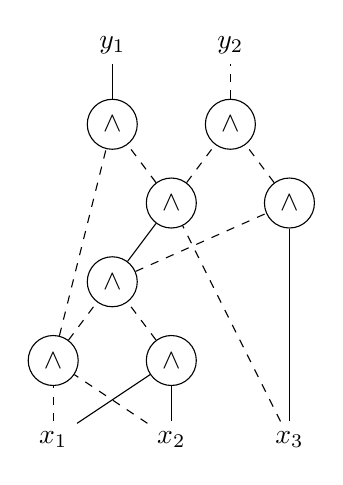
\begin{tikzpicture}[]
    % First rank with three nodes called x_1, x_2, x_3
    \node[draw=none] (x_1) at (0,0) {$x_1$};
    \node[draw=none] (x_2) at (1.5,0) {$x_2$};
    \node[draw=none] (x_3) at (3,0) {$x_3$};
    
    % Second rank with two nodes above x_1 and x_2 called x_4, x_5
    \node[draw, circle] (x_4) at (0.00, 1) {$\land$};
    \node[draw, circle] (x_5) at (1.50, 1) {$\land$};
    
    % Third rank with one node called x_6
    \node[draw, circle] (x_6) at (0.75, 2) {$\land$};

    % Fourth rank with two nodes called x_7 and x_8
    \node[draw, circle] (x_7) at (1.5, 3) {$\land$};
    \node[draw, circle] (x_8) at (3, 3) {$\land$};

    % Fifth rank with two nodes called x_9 and x_10
    \node[draw, circle] (x_9) at  (0.75,4) {$\land$};
    \node[draw, circle] (x_10) at (2.25,4) {$\land$};

    % Sixth rank with two nodes called y_1 and y_2
    \node[draw=none] (y_1) at (0.75,5) {$y_1$};
    \node[draw=none] (y_2) at (2.25,5) {$y_2$};
    
    % Connections
    \draw[dashed] (x_1) -- (x_4);
    \draw (x_1) -- (x_5);
    
    \draw[dashed] (x_2) -- (x_4);
    \draw (x_2) -- (x_5);

    \draw[dashed] (x_3) -- (x_7);
    \draw (x_3) -- (x_8);

    \draw[dashed] (x_4) -- (x_9);
    \draw[dashed] (x_4) -- (x_6);

    \draw[dashed] (x_5) -- (x_6);

    \draw (x_6) -- (x_7);
    \draw[dashed] (x_6) -- (x_8);

    \draw[dashed] (x_7) -- (x_9);
    \draw[dashed] (x_7) -- (x_10);

    \draw[dashed] (x_8) -- (x_10);

    \draw (x_9) -- (y_1);

    \draw[dashed] (x_10) -- (y_2);
    
\end{tikzpicture}


\subsubsection{Structural Properties: Levels, Logic Cones, Fanout}
\label{sec:prelim:aig:properties}
The topological level of a node is its longest distance from the input frontier,
\begin{equation}
    \ell(v) =
    \begin{cases}
        0 & \text{if } \operatorname{fi}(v) = \emptyset, \\[2pt]
        1 + \max_{u \in \operatorname{fi}(v)} \ell(u) & \text{otherwise,}
    \end{cases}
    \label{eq:prelim:level}
\end{equation}
and the depth of the graph is $\ell(G) = \max_{v \in \mathcal{V}} \ell(v)$, an absolute
coordinate an AIG carries and a general graph does not, read by the positional encoding
(\ref{sec:method:data:representation:pe}), the level-sliced and span-weighted partitioners
(\ref{sec:method:reduction:partitioning}), and the cone candidate
(\ref{sec:method:summary:domain}).

% The topological level of a node is its longest distance from the input frontier, and the
% depth of the graph is $\ell(G) = \max_{v \in \mathcal{V}} \ell(v)$. The drawn height of a
% gate in~\ref{fig:aig_example} is exactly $\ell$. Level is an absolute coordinate that an AIG
% has and a general graph does not, and four constructions in this thesis read it: the
% positional encoding of~\ref{sec:method:data:representation:pe}, the level slicing and
% span-weighted partitioners of~\ref{sec:method:reduction:partitioning}, and the level bands
% of the cone candidate in~\ref{sec:method:summary:domain}.

Writing $u \rightsquigarrow v$ for a directed path, of length zero when $u = v$, the fanin
cone (the logic or causal cone) and fanout cone of $v$ are
\begin{equation}
    \mathcal{C}(v) = \{\, u \in \mathcal{V} : u \rightsquigarrow v \,\},
    \qquad
    \mathcal{F}(v) = \{\, w \in \mathcal{V} : v \rightsquigarrow w \,\}.
    \label{eq:prelim:cone}
\end{equation}
The claim of~\ref{sec:intro:motivation:reduction}, that generic reduction severs causal
structure, is a claim about $\mathcal{C}$: deleting one edge on a long path removes gates from
every downstream cone, regardless of similarity under an undirected measure. The
depth-bounded form $\mathcal{C}_k$ of~\eqref{eq:method:cone} makes the effect measurable.

% Writing $u \rightsquigarrow v$ for the existence of a directed path, of length zero when
% $u = v$, the fanin cone (equivalently the logic or causal cone) and the fanout cone of $v$
% are Both cones contain $v$ itself. The fanin cone is the set of gates on which $v$
% functionally depends, and~\eqref{eq:prelim:level} measures the longest path through it. The
% claim of~\ref{sec:intro:motivation:reduction}, that generic reduction severs causal
% structure, is a claim about $\mathcal{C}$: deleting one edge on a long path removes gates
% from the cones of everything downstream of it, whether or not the result resembles the
% original under an undirected measure. The depth-bounded form $\mathcal{C}_k$
% of~\eqref{eq:method:cone} is what makes the effect measurable.

Fanout degree $|\operatorname{fo}(v)|$ separates gates consumed once from gates shared and
reused, which constrains rewriting. Reconvergence is the same property from below: $v$ is a
reconvergence point of $u$ when two internally disjoint paths run from $u$ to $v$. AIGs are
dense in reconvergence: structural hashing (\ref{sec:prelim:algorithms:primitives}) shares
duplicated subexpressions rather than replicating them \citep{kuehlmann2002robust}.

% Fanout degree $|\operatorname{fo}(v)|$ separates gates whose output is consumed once from
% gates whose output is shared. Chains of single-fanout gates carry no sharing information;
% multi-fanout gates are the points at which logic is reused, and they are what constrains
% rewriting. Reconvergence is the same property seen from below: $v$ is a reconvergence point
% of $u$ when two internally disjoint directed paths run from $u$ to $v$. AIGs are dense in
% reconvergence, because structural hashing (\ref{sec:prelim:algorithms:primitives}) shares
% every duplicated subexpression instead of replicating it \citep{kuehlmann2002robust}.

Where a fanout cone reconverges is a question of post-dominance
\citep{lengauer1979dominators}. Appending a virtual sink $t$ after every PO and extending
$\prec$ to it, the immediate post-dominator of $v$ is
\begin{equation}
    \operatorname{ipdom}(v) = \min_{\prec}
        \{\, u \neq v : \text{every } v \rightsquigarrow t \text{ path meets } u \,\},
    \label{eq:prelim:ipdom}
\end{equation}
the gate at which $\mathcal{F}(v)$ reconverges, or $t$ when it never does. The cone
candidate of~\ref{sec:method:summary:domain} groups gates by $\operatorname{ipdom}$.

The Maximal Fanout-Free Cone (MFFC) of a root gate $v$ collects the gates feeding $v$ and
nothing else \citep{mishchenko2006rewriting},
\begin{equation}
    \operatorname{MFFC}(v) = \{\, u \in \mathcal{C}(v) :
        \text{every path } u \rightsquigarrow t \text{ passes through } v \,\},
    \label{eq:prelim:mffc}
\end{equation}
so removing $v$ removes exactly $\operatorname{MFFC}(v)$: the unit refactoring re-expresses
one at a time (\ref{sec:prelim:algorithms:primitives}) and the second domain candidate
merges (\ref{sec:method:summary:domain}).

% The Maximal Fanout-Free Cone (MFFC) of a root gate $v$ collects the gates feeding $v$ and
% nothing else, so removing $v$ from the network removes exactly $\operatorname{MFFC}(v)$ and
% nothing more. That property makes the MFFC the natural unit of local restructuring, and
% refactoring collapses and re-expresses one MFFC at a time
% (\ref{sec:prelim:algorithms:primitives}). It is also the unit merged by the second domain
% candidate of~\ref{sec:method:summary:domain}, which is why that candidate carries an
% argument about label leakage and the others do not.

\subsubsection{Why AIGs Differ from General Graphs}
\label{sec:prelim:aig:distinct}
Five properties separate an AIG from the citation, social and knowledge graphs on which graph
reduction was developed, and each costs a generic method something specific.

(i) An AIG is directed and acyclic: reducing on the undirected projection discards the
orientation that carries the logic, since a DAG's quotient need not itself be acyclic, as in
the spanning forest of~\ref{sec:method:sparse:forest}.

% (i) An AIG is directed and acyclic. Machinery built for undirected graphs does not transfer
% unchanged, because a quotient of a DAG need not be acyclic, and a reduction computed on the
% undirected projection discards the orientation that carries the logic. The spanning forest
% of~\ref{sec:method:sparse:forest} is the concrete case.

(ii) Depth, not width, is the binding dimension: the critical path (longest PI-to-PO path)
has length $\ell(G)$ of~\eqref{eq:prelim:level}, the quantity balancing shortens
(\ref{sec:prelim:algorithms:primitives}) and an encoder must span. After $L$
message-passing layers a node depends only on its $L$-hop neighbourhood
(\ref{sec:prelim:gnn:mp}), so $\mathcal{C}_L(v) = \mathcal{C}(v)$ only when
\begin{equation}
    L \ge \ell(v).
    \label{eq:prelim:reach}
\end{equation}
Corpus depth is $35$ levels at the median and $24{,}802$ at the maximum
(\ref{sec:method:data:sources}) against a single-digit encoder depth, so~\eqref{eq:prelim:reach}
holds only near the input frontier: receptive-field starvation is the normal condition here,
which hypothesis H1 (\ref{sec:intro:rq3}) proposes coarsening relieves.

% (ii) Depth, not width, is the binding dimension. The critical path is a longest directed
% path from a PI to a PO, and its length is the depth $\ell(G)$ of~\eqref{eq:prelim:level}:
% the quantity balancing exists to shorten (\ref{sec:prelim:algorithms:primitives}) and the
% quantity an encoder has to span. After $L$ message-passing layers a node representation
% depends on its $L$-hop neighbourhood and on nothing else (\ref{sec:prelim:gnn:mp}), so a
% gate reads the whole of the logic it depends on, $\mathcal{C}_L(v) = \mathcal{C}(v)$, only
% when Corpus depth is $35$ levels at the median and $24{,}802$ at the maximum
% (\ref{sec:method:data:sources}), against an encoder depth in single digits,
% so~\eqref{eq:prelim:reach} holds only near the input frontier. Receptive-field starvation is
% the normal condition on this data, and it is the starvation that hypothesis H1
% (\ref{sec:intro:rq3}) proposes coarsening relieves.

(iii) Edges carry function: the inversion in~\eqref{eq:prelim:inversion} is part of what the
graph represents, so averaging or discarding $\mathrm{inv}$ changes the Boolean function
rather than approximating it, unlike every summarization method here, which keeps normal and
inverted connections distinguishable.

% (iii) Edges carry function. The inversion in~\eqref{eq:prelim:inversion} is part of what
% the graph represents, so a merge that averages or discards $\mathrm{inv}$ changes the
% Boolean function rather than approximating it. Every summarization method here is therefore
% constrained to keep normal and inverted connections distinguishable, a constraint no
% general method imposes on itself.

(iv) The interface is fixed: the PIs and POs are the circuit's contract with the rest of the
design, so merging them away changes what the graph is rather than coarsening it
(\ref{sec:method:summary:mergemap}).

% (iv) The interface is fixed. The PIs and POs are the circuit's contract with the
% rest of the design, and merging them away changes what the graph is rather than coarsening
% it. The boundary is enforced uniformly in~\ref{sec:method:summary:mergemap}.

(v) Node count is at once the cost and the scale of the label. Fanin cardinality is fixed by
the basis, so
\begin{equation}
    |\mathcal{E}| = 2 \left| \tau^{-1}(\mathrm{AND}) \right|
        + \left| \tau^{-1}(\mathrm{PO}) \right| < 2 \left| \mathcal{V} \right|,
    \label{eq:prelim:edges}
\end{equation}
and one message-passing layer costs $\Theta(|\mathcal{V}|)$ at fixed width: an AIG carries no
surplus density, so removing edges alone cannot lower that cost at any retention ratio
(\ref{sec:prelim:reduction:sparsification}). The same count is the optimizability
target's~\eqref{eq:prelim:target} denominator, so $y(G)$ is quantised in steps of
$1/|\mathcal{V}(G)|$, coarsest on the smallest circuits, where the corpus piles up at exactly
zero (\ref{sec:method:data:statistics:label}).

% (v) Node count is at once the cost and the scale of the label. Fanin cardinality is fixed
% by the basis, so and one message-passing layer therefore costs $\Theta(|\mathcal{V}|)$ at
% fixed width. An AIG carries no surplus density, so removing edges alone cannot take that
% cost below the same order at any retention ratio
% (\ref{sec:prelim:reduction:sparsification}). The same count is the denominator of the
% optimizability target~\eqref{eq:prelim:target}, so $y(G)$ is quantised in steps of
% $1/|\mathcal{V}(G)|$ and is coarsest on the smallest circuits, which is where the corpus
% piles up at exactly zero (\ref{sec:method:data:statistics:label}).

A reduction operator can respect or ignore the first four at no syntactic cost. Whether
respecting them buys accuracy is the question RQ4 (\ref{sec:intro:rq4}) measures.
